\documentclass[11pt]{article}
\usepackage[margin=27mm]{geometry}\usepackage{pdfpages,hyperref}
\pdfinclusioncopyfonts=1
\begin{document}
\begin{center}{\Large Rank two projective geometries}\\[4mm]
{\large Complete source treatment and shared proofs for L063 and L064}\end{center}
The published Part II article and the retained appendix are separately
registered originals. Their individual claim ledgers accompany this
volume. The opening manuscript identifies every correction and the
classical premises; the following papers contain the full proofs.
The omitted affine family and all previously accepted components are
reused without repeating their acquisition. Earlier scope statements
inside those exact components retain their historical wording; the
opening manuscript records their completed source joins. No new
principal-refutation count, compression ratio or Lean verification is
claimed.\par\medskip
\small\begin{tabular}{rp{.84\textwidth}}
2 & Source treatment, corrected formulas and attribution\\
8 & The omitted affine configurations\\
11 & Two-transitive coset actions in dimension two\\
17 & Subfield planes and unordered pairs of parabolics\\
22 & Counting configurations above a cyclic subgroup of order three\\
26 & Exceptional parabolics from their common normalizers\\
30 & Subfield parabolics and affine overgroups\\
37 & Local arc transitivity from small stabilizers\\
43 & Full automorphisms of the dihedral subdivision family\\
46 & Pairs of symmetric parabolics and their full graph groups\\
50 & The order-nine geometry from pairs and matchings\\
\end{tabular}\newpage
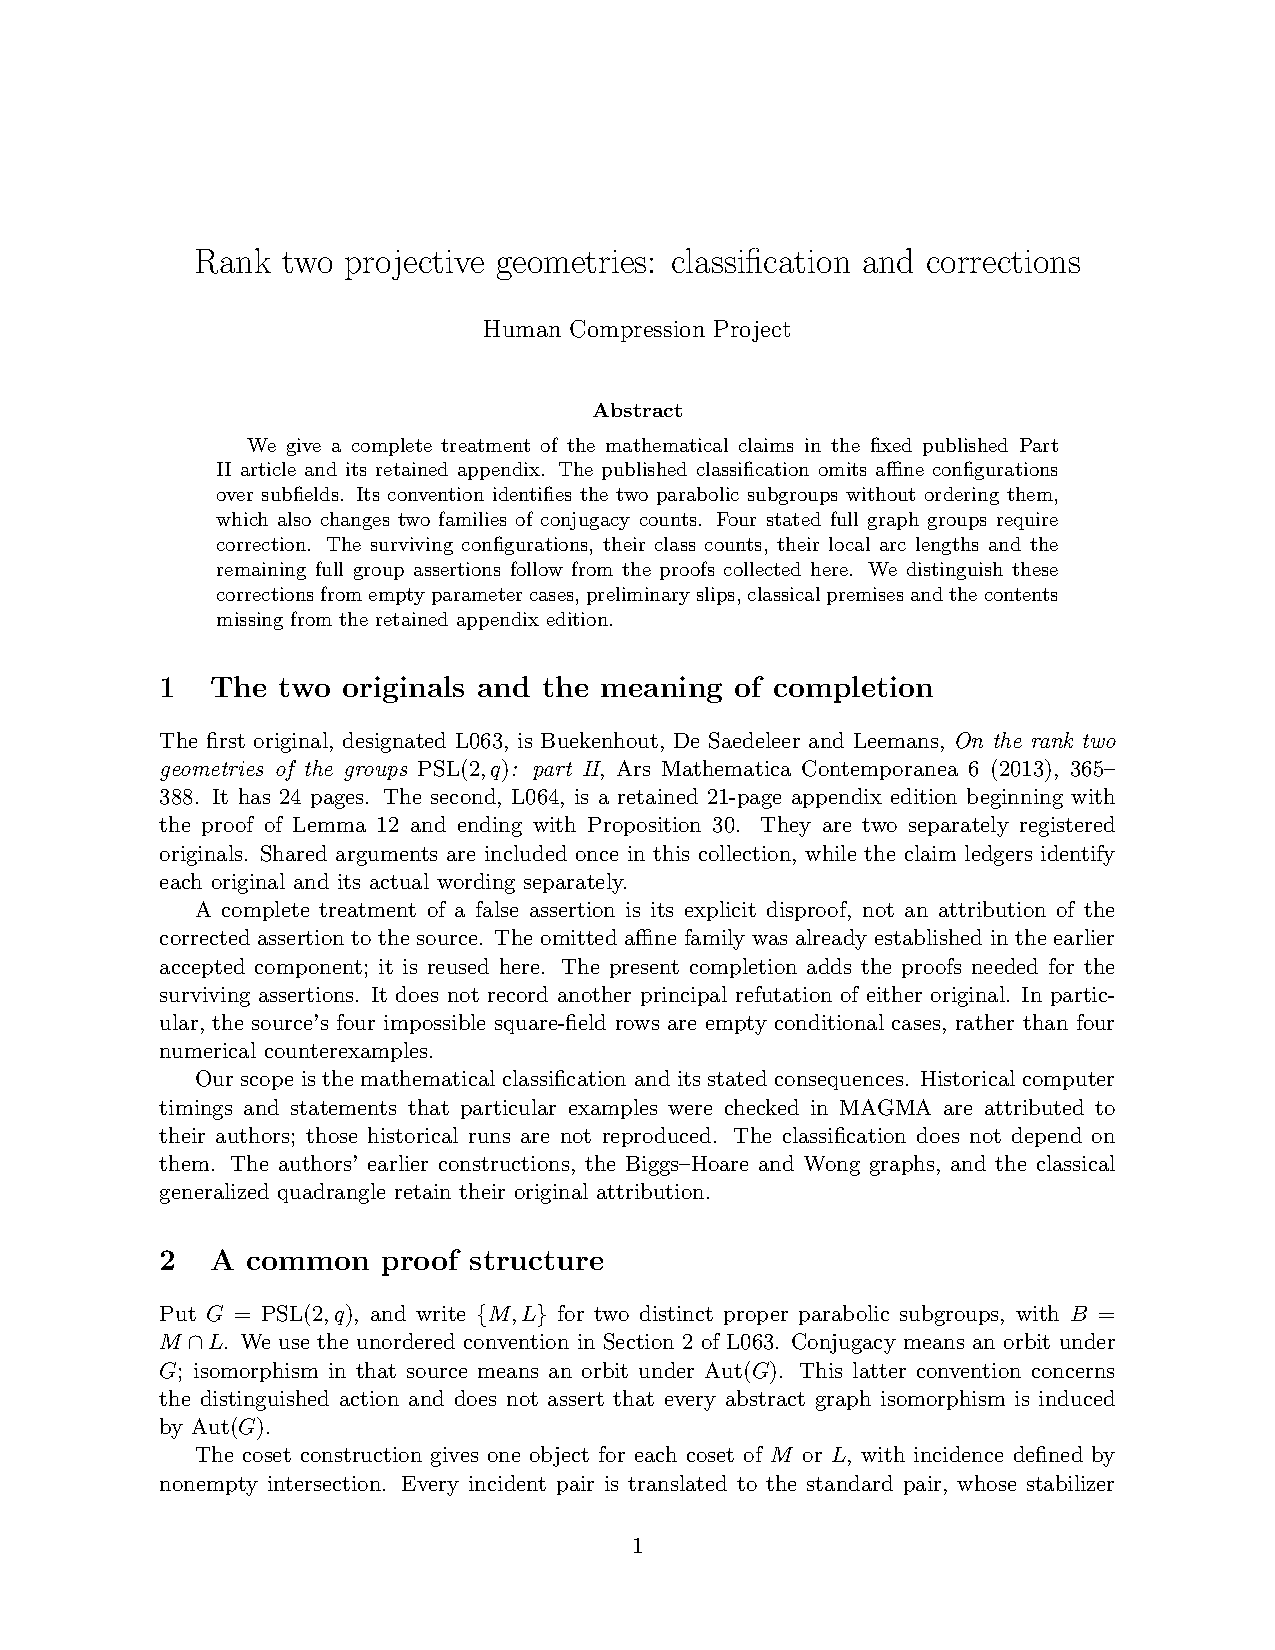
\includepdf[pages=-]{completion.pdf}
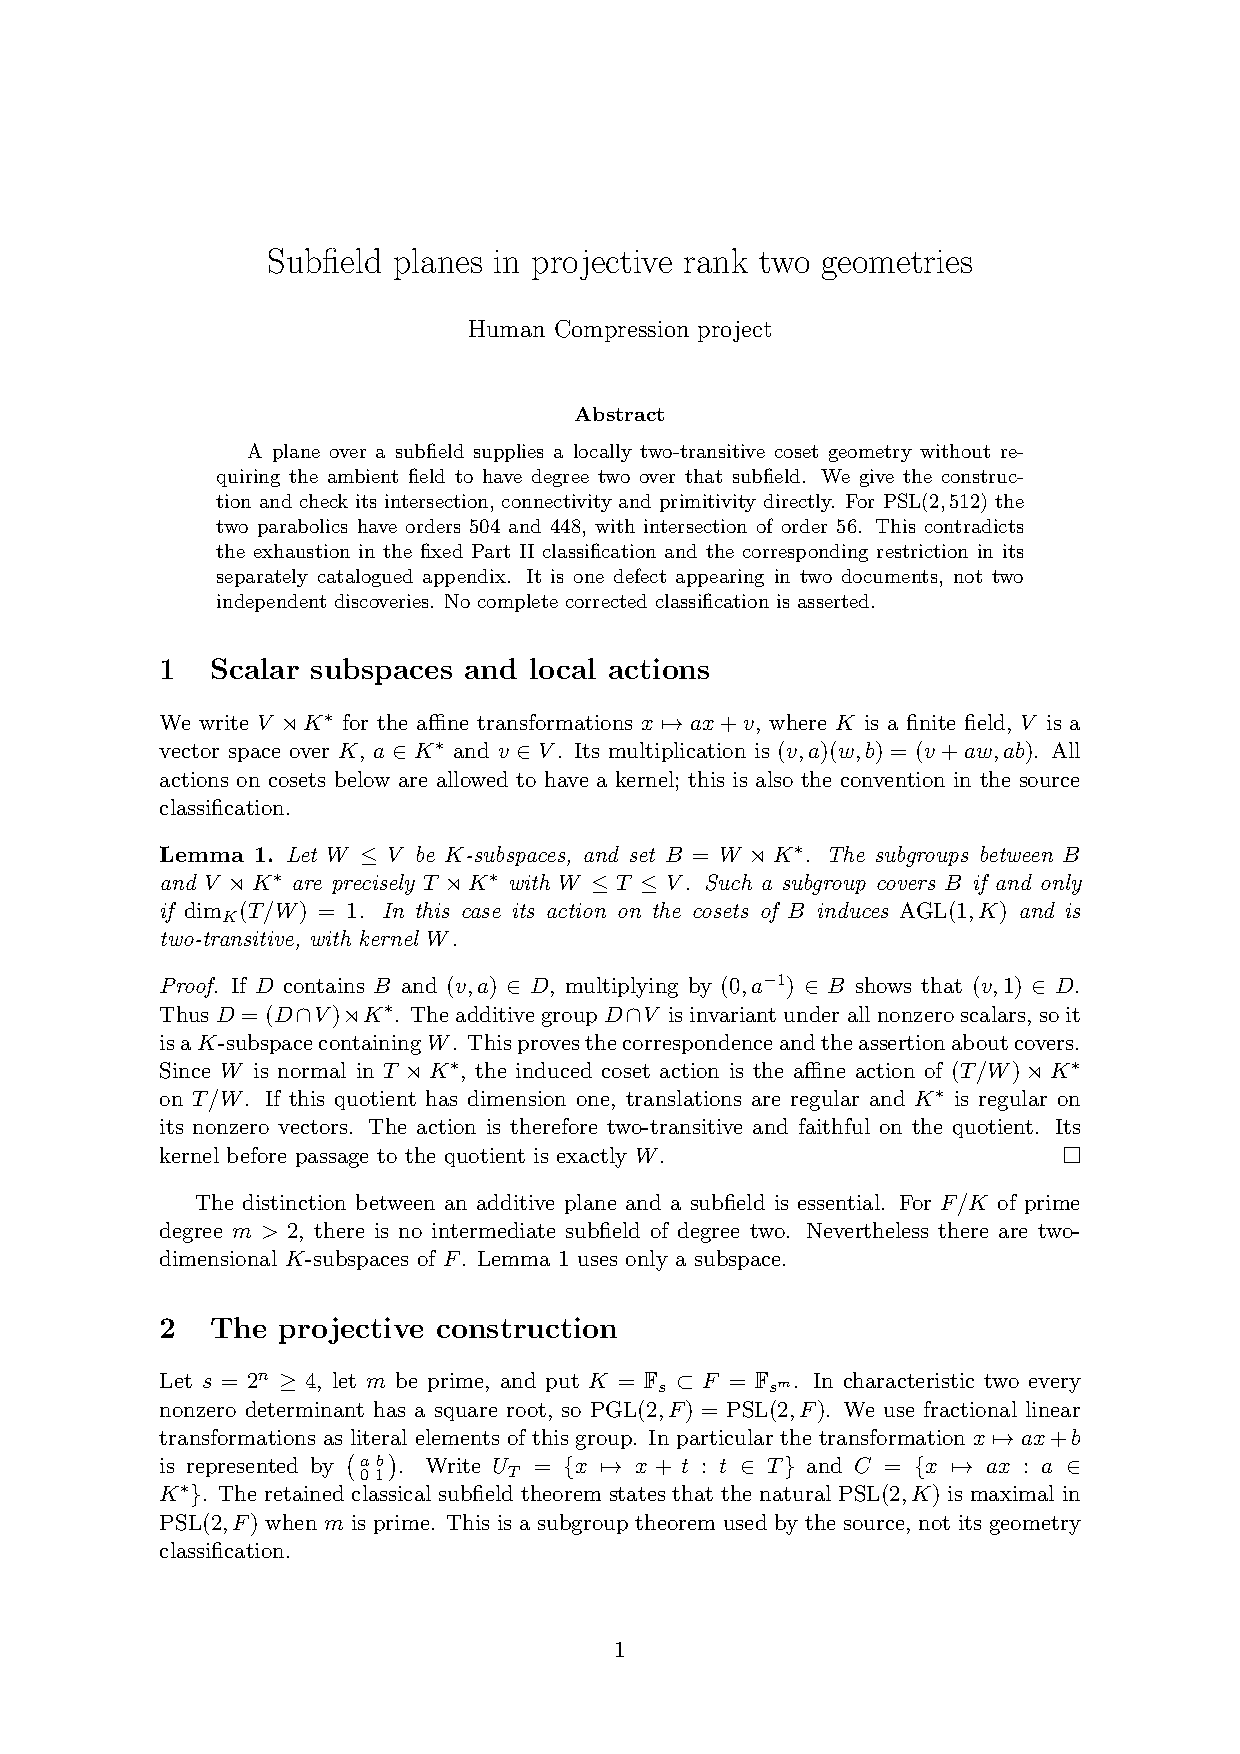
\includepdf[pages=-]{proofs/omitted_affine.pdf}
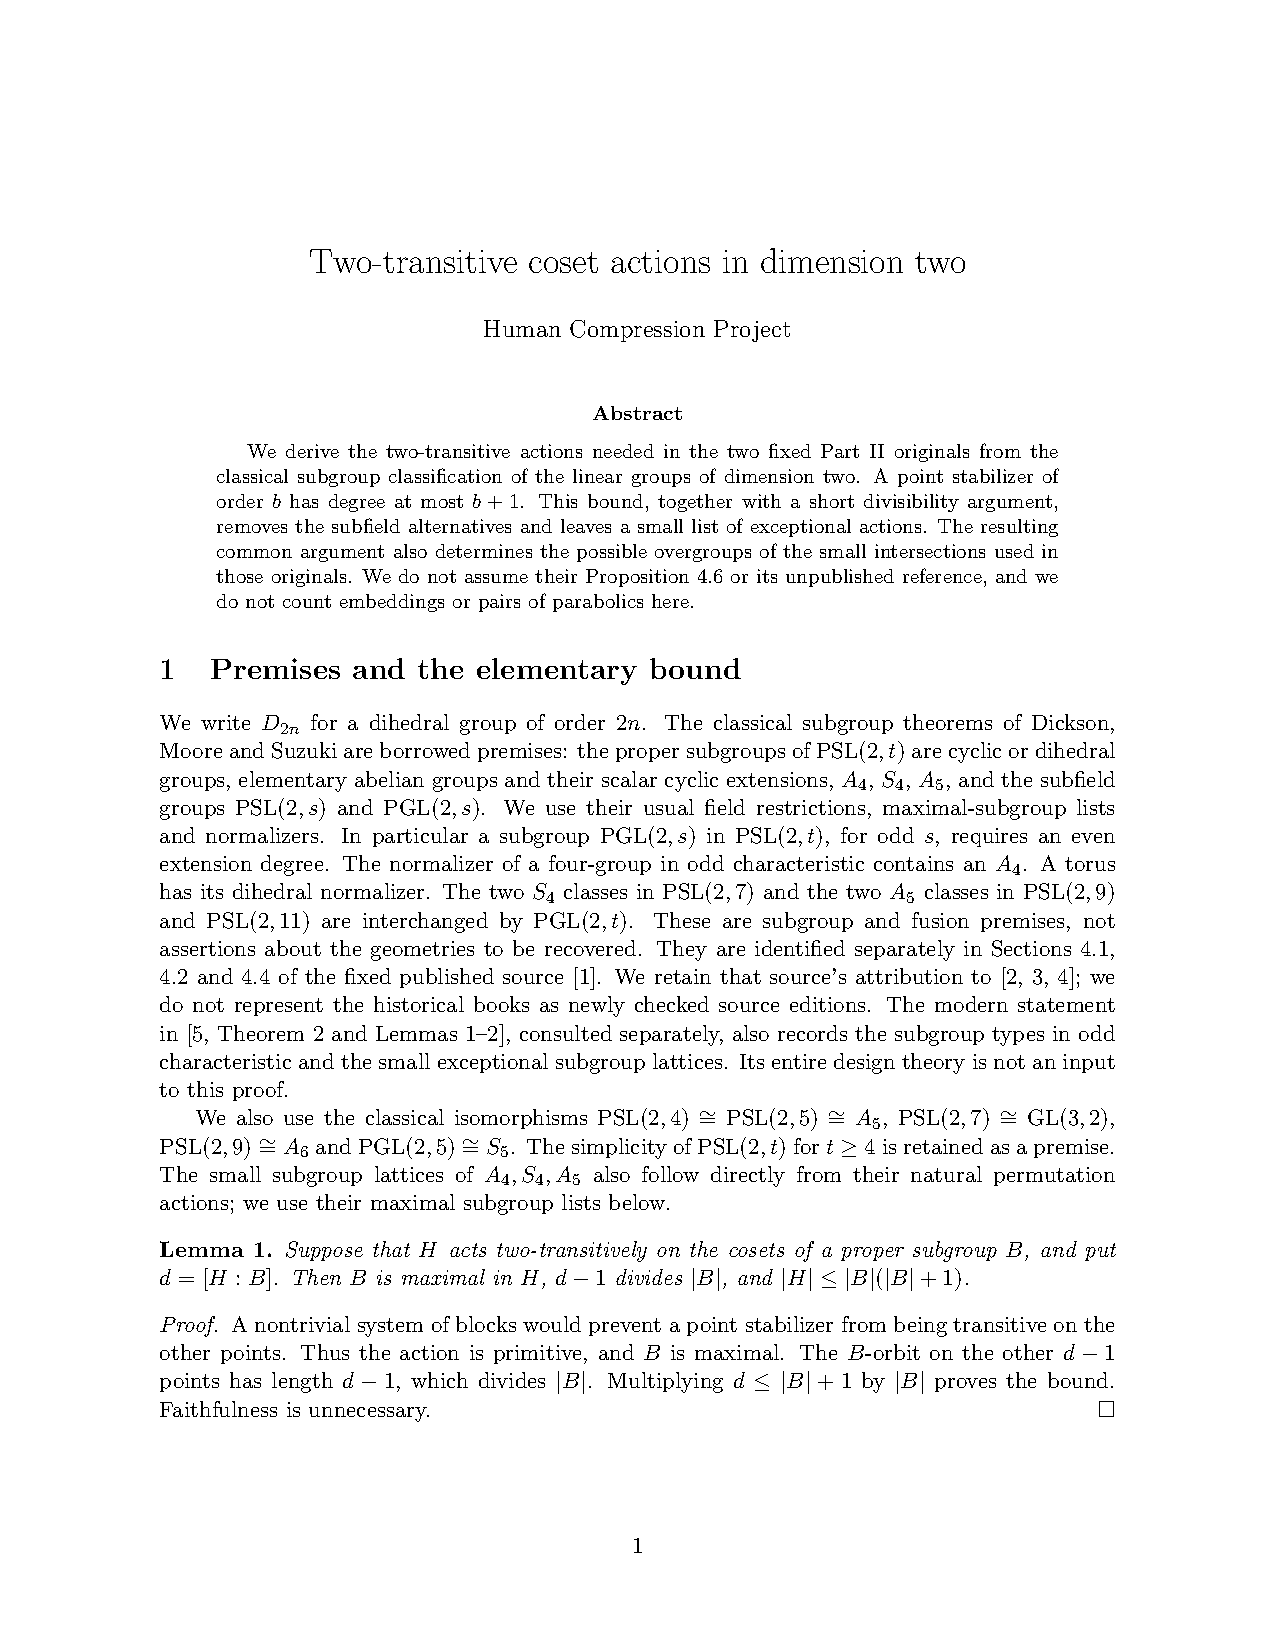
\includepdf[pages=-]{proofs/overgroups.pdf}
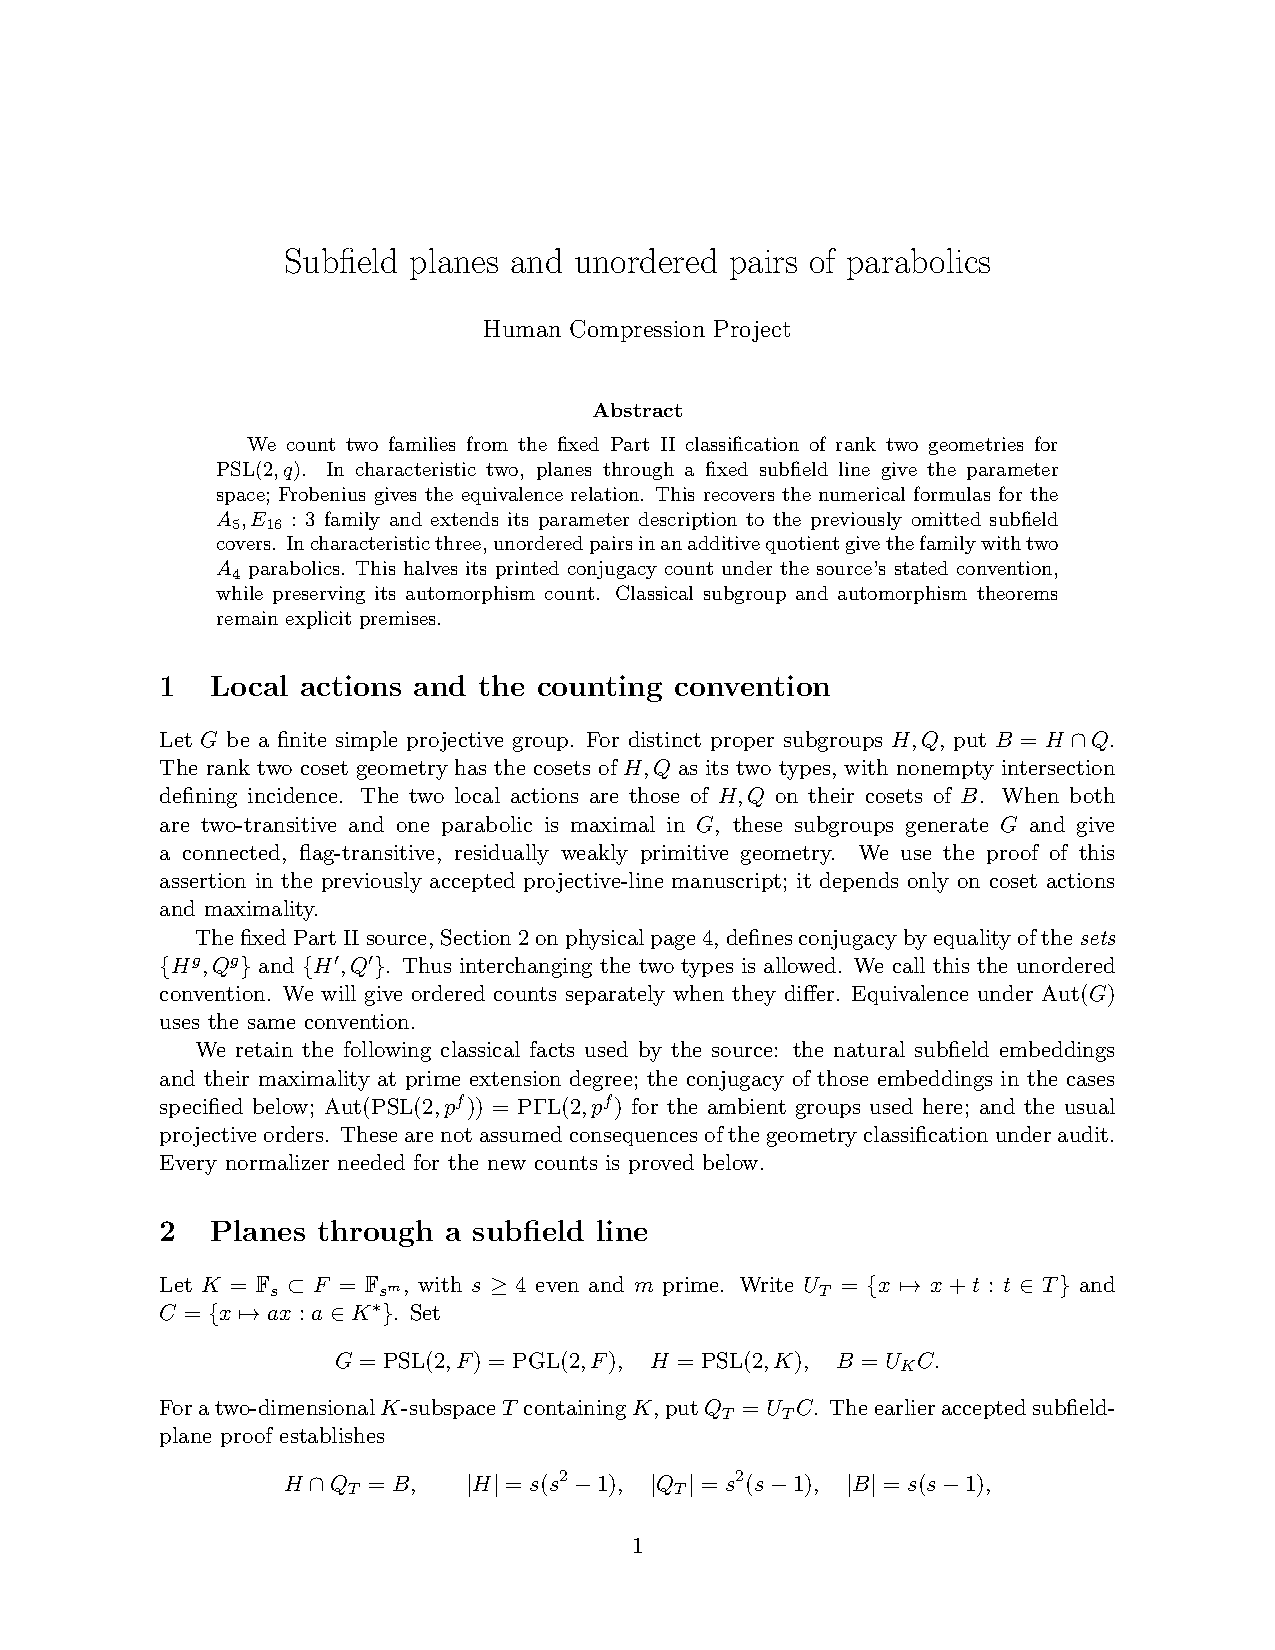
\includepdf[pages=-]{proofs/scalar.pdf}
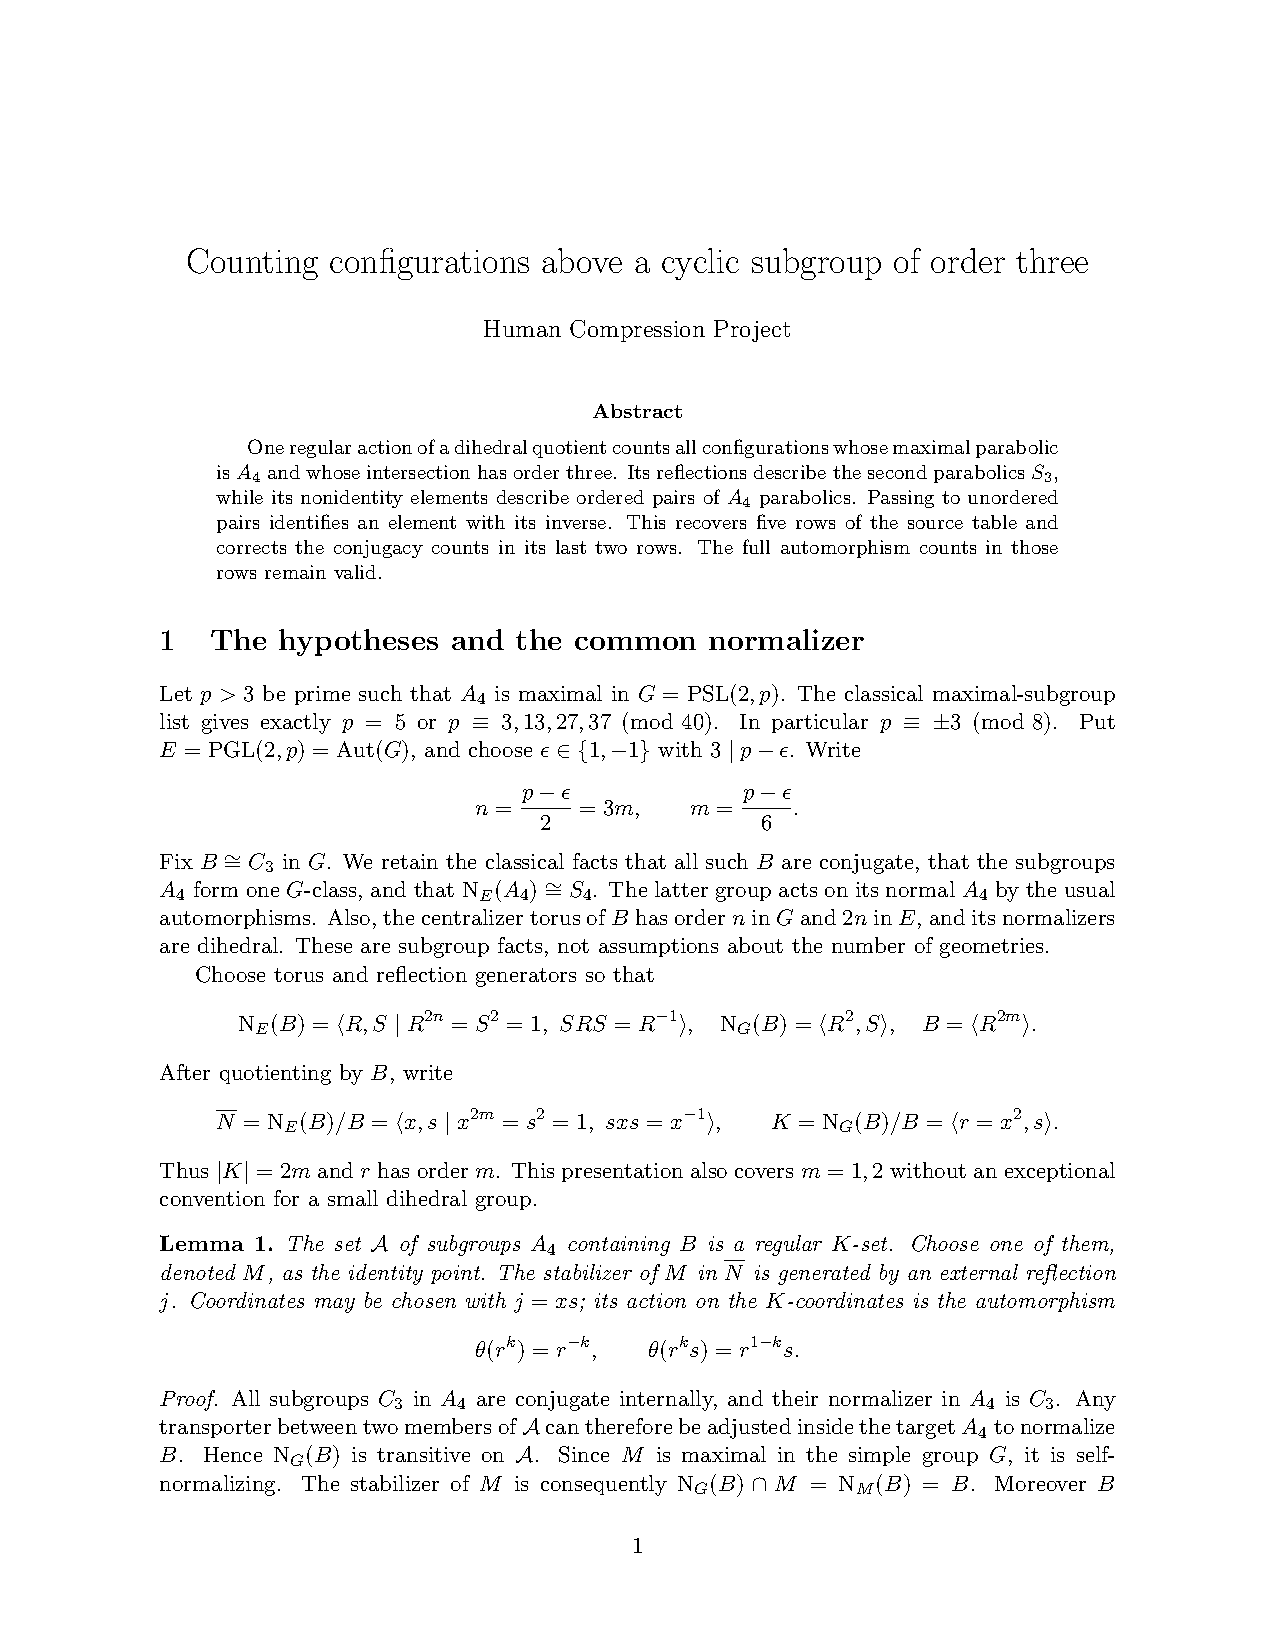
\includepdf[pages=-]{proofs/cyclic_three.pdf}
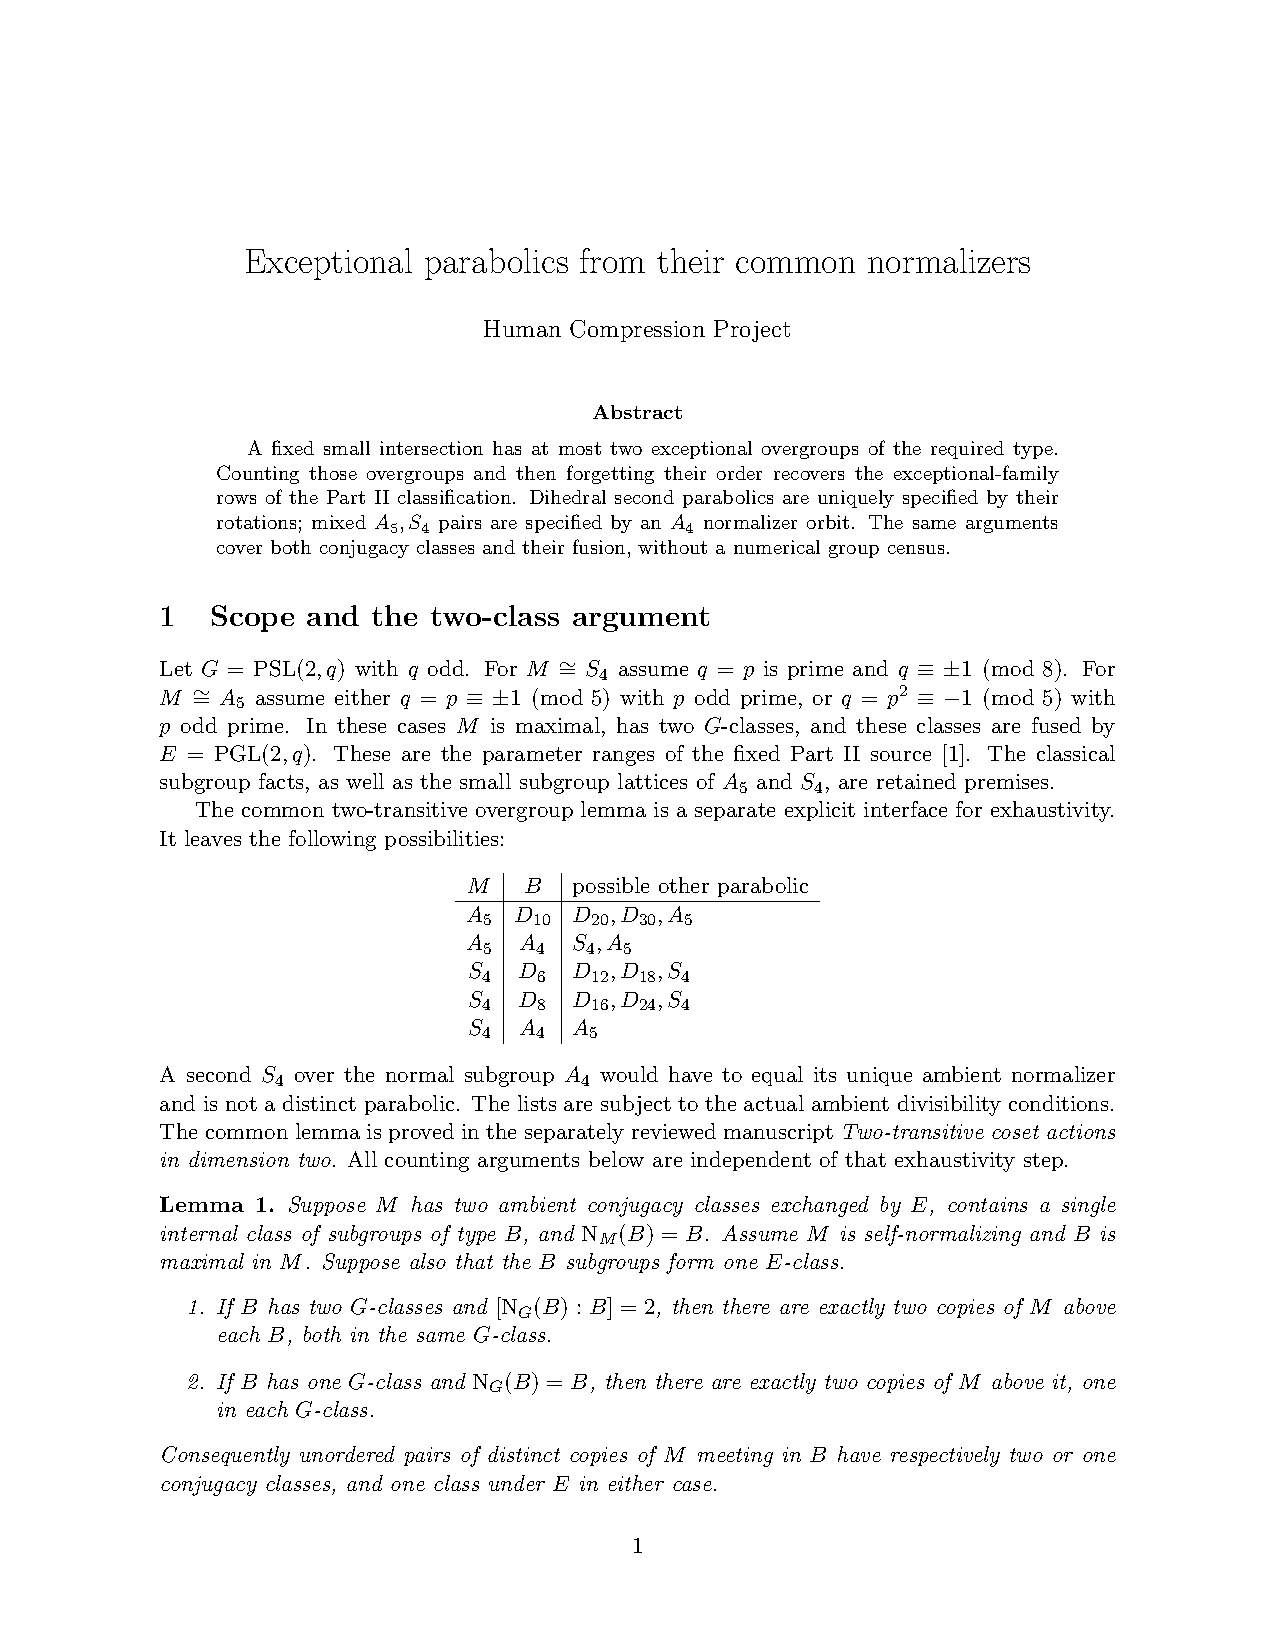
\includepdf[pages=-]{proofs/exceptional.pdf}
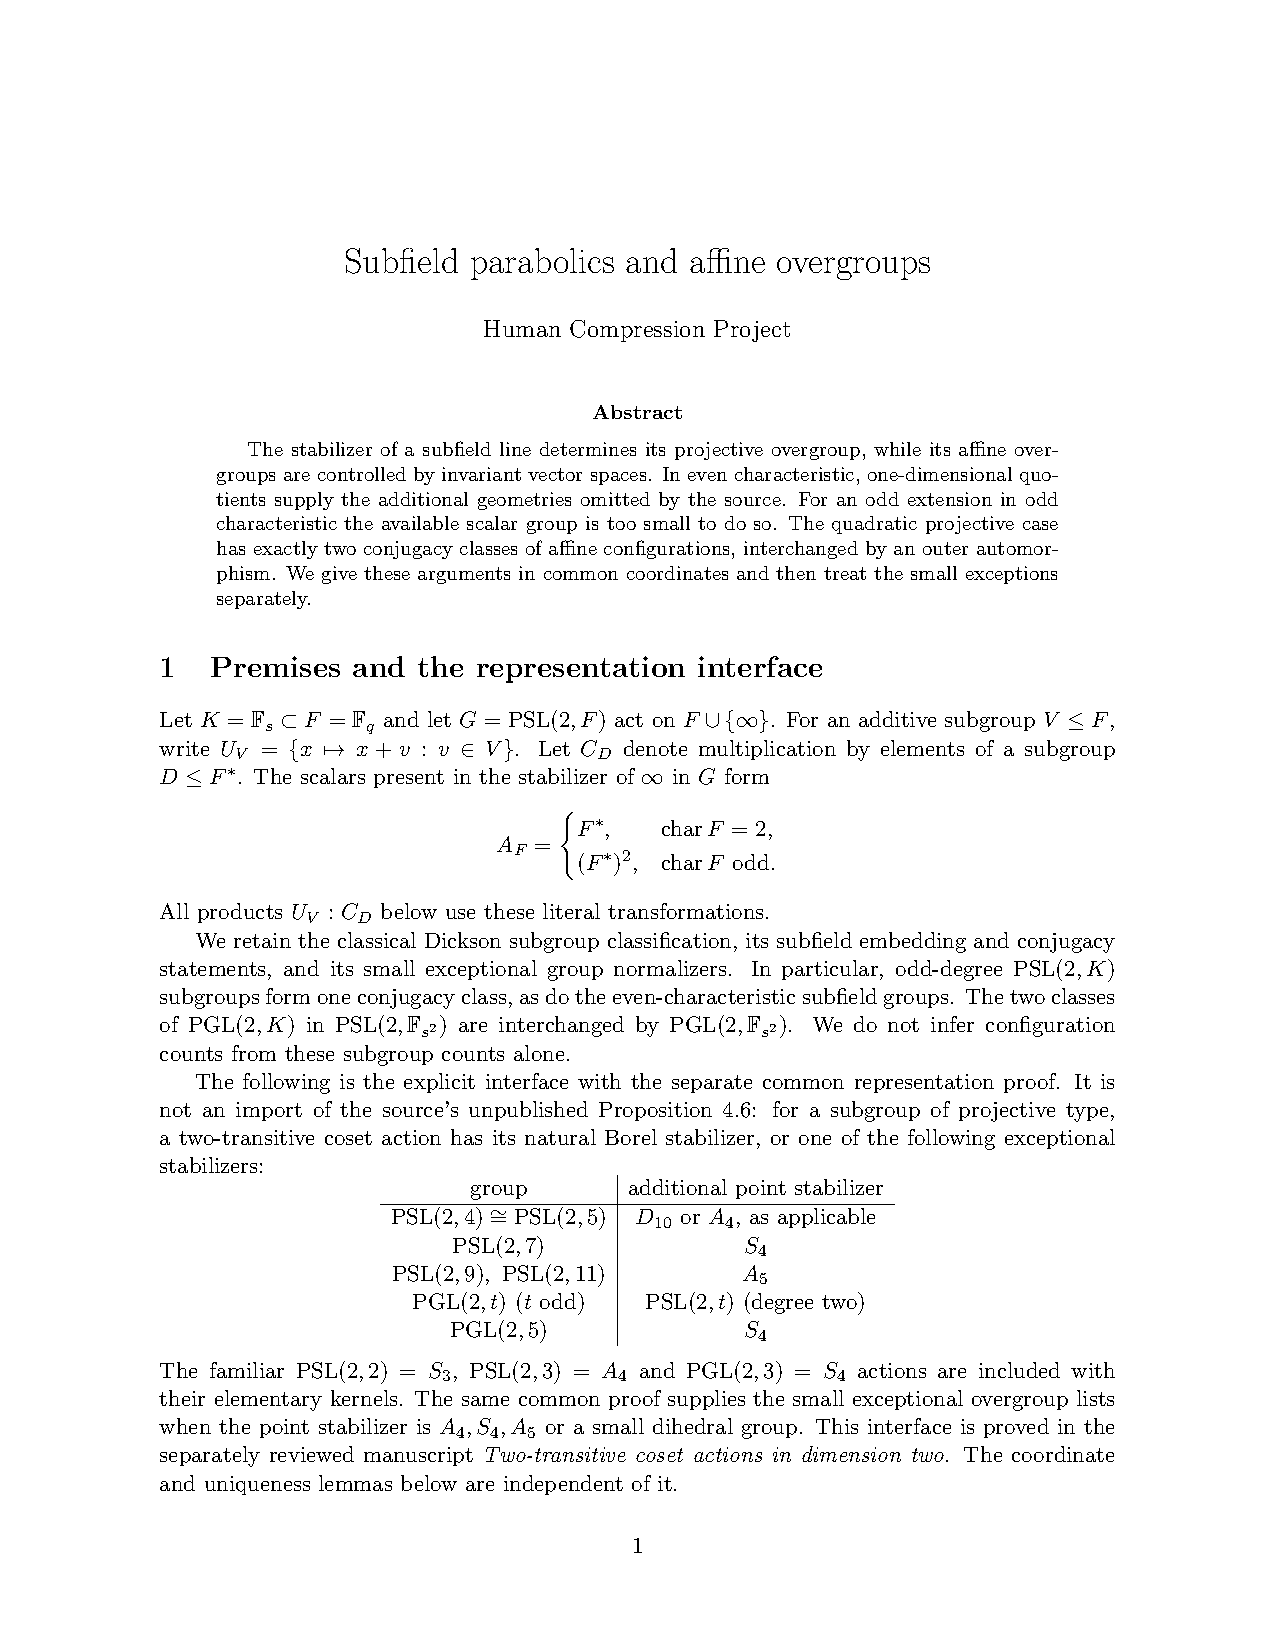
\includepdf[pages=-]{proofs/subfields.pdf}
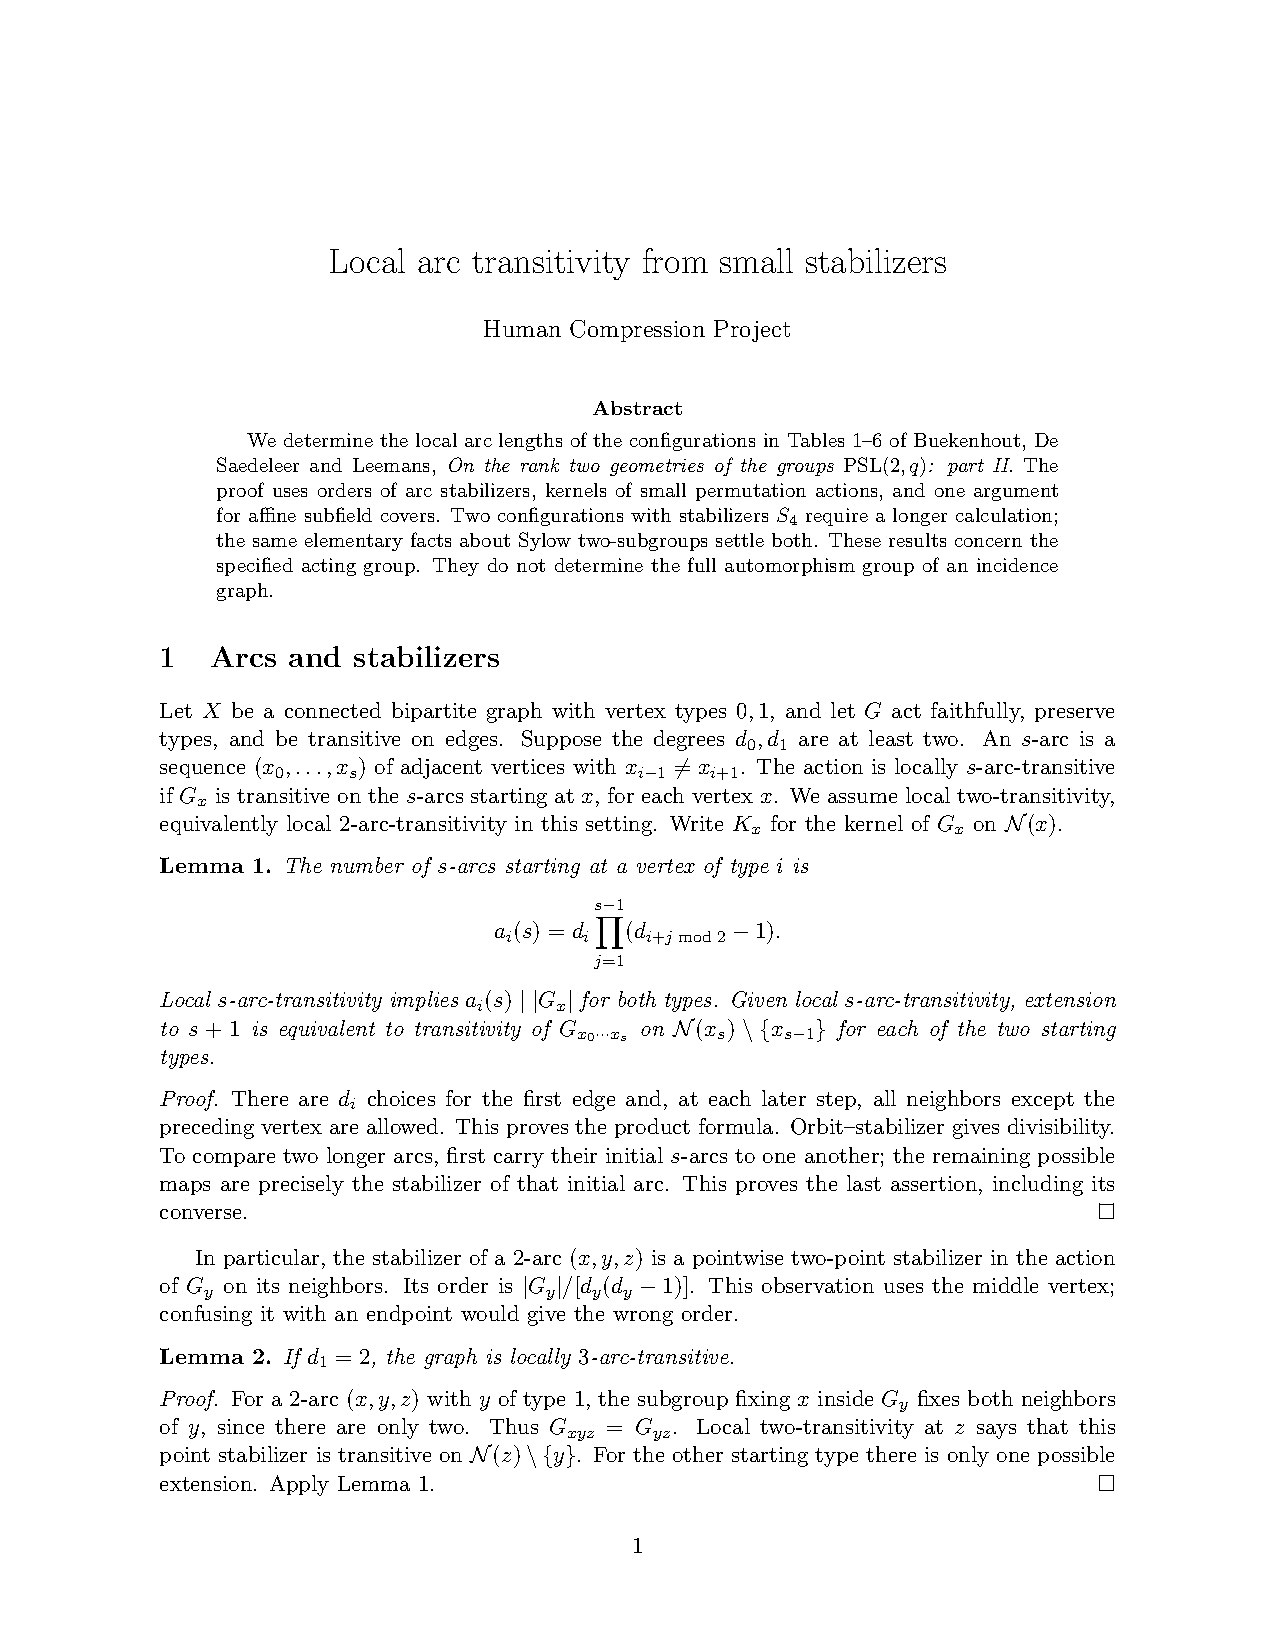
\includepdf[pages=-]{proofs/arcs.pdf}
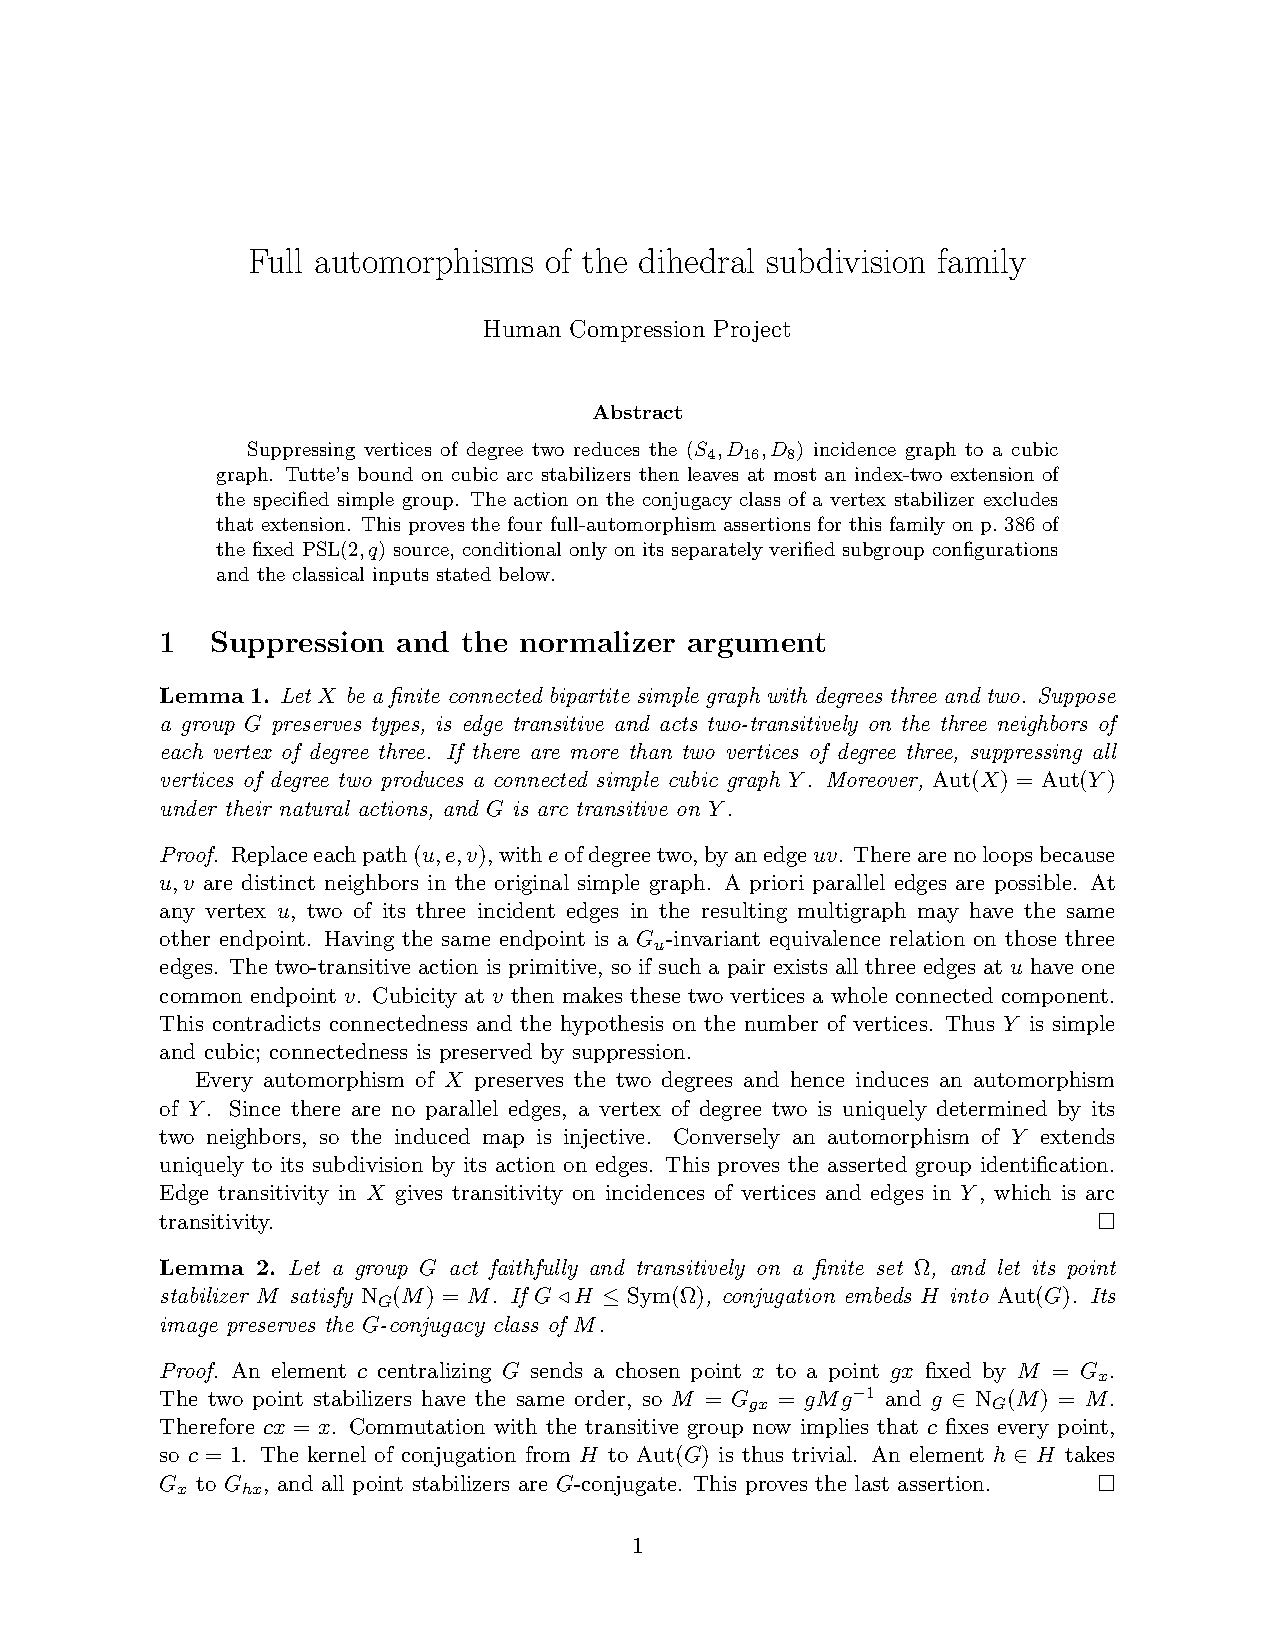
\includepdf[pages=-]{proofs/subdivision.pdf}
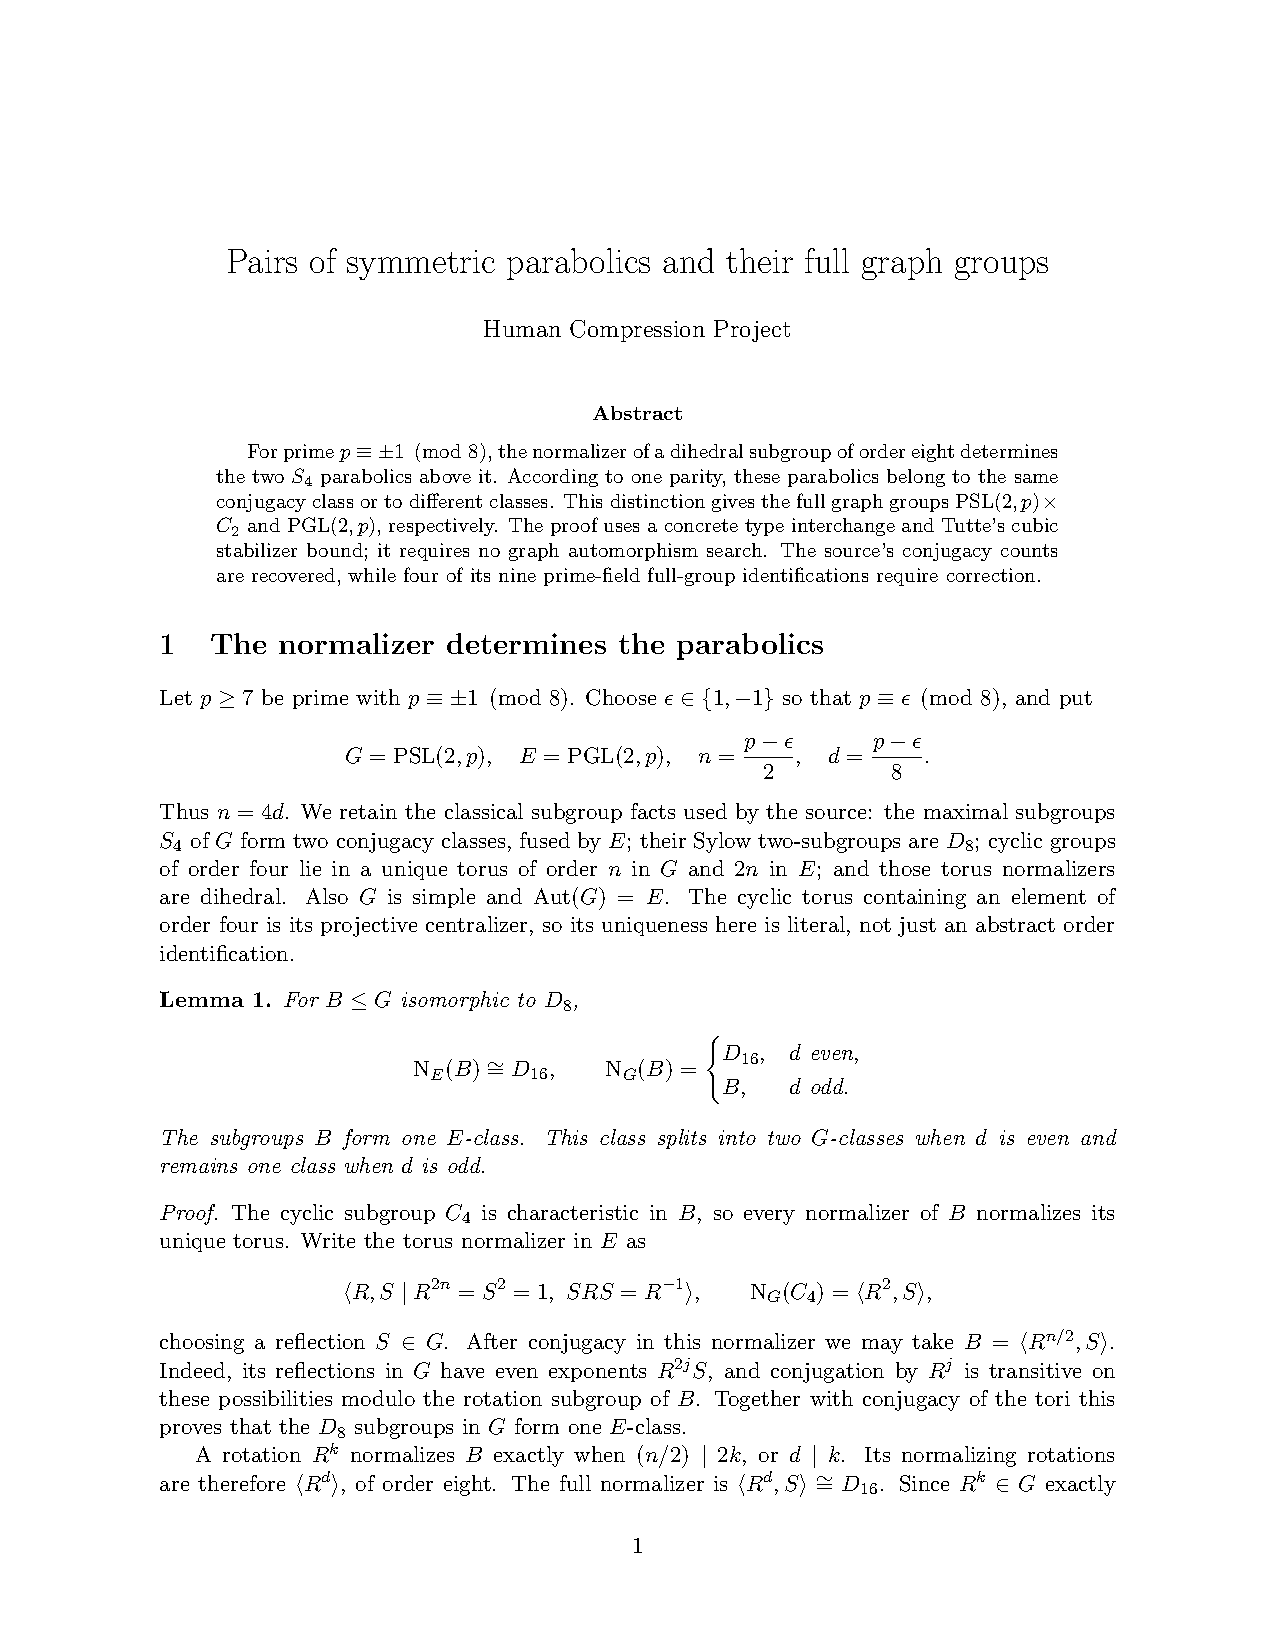
\includepdf[pages=-]{proofs/s4_pairs.pdf}
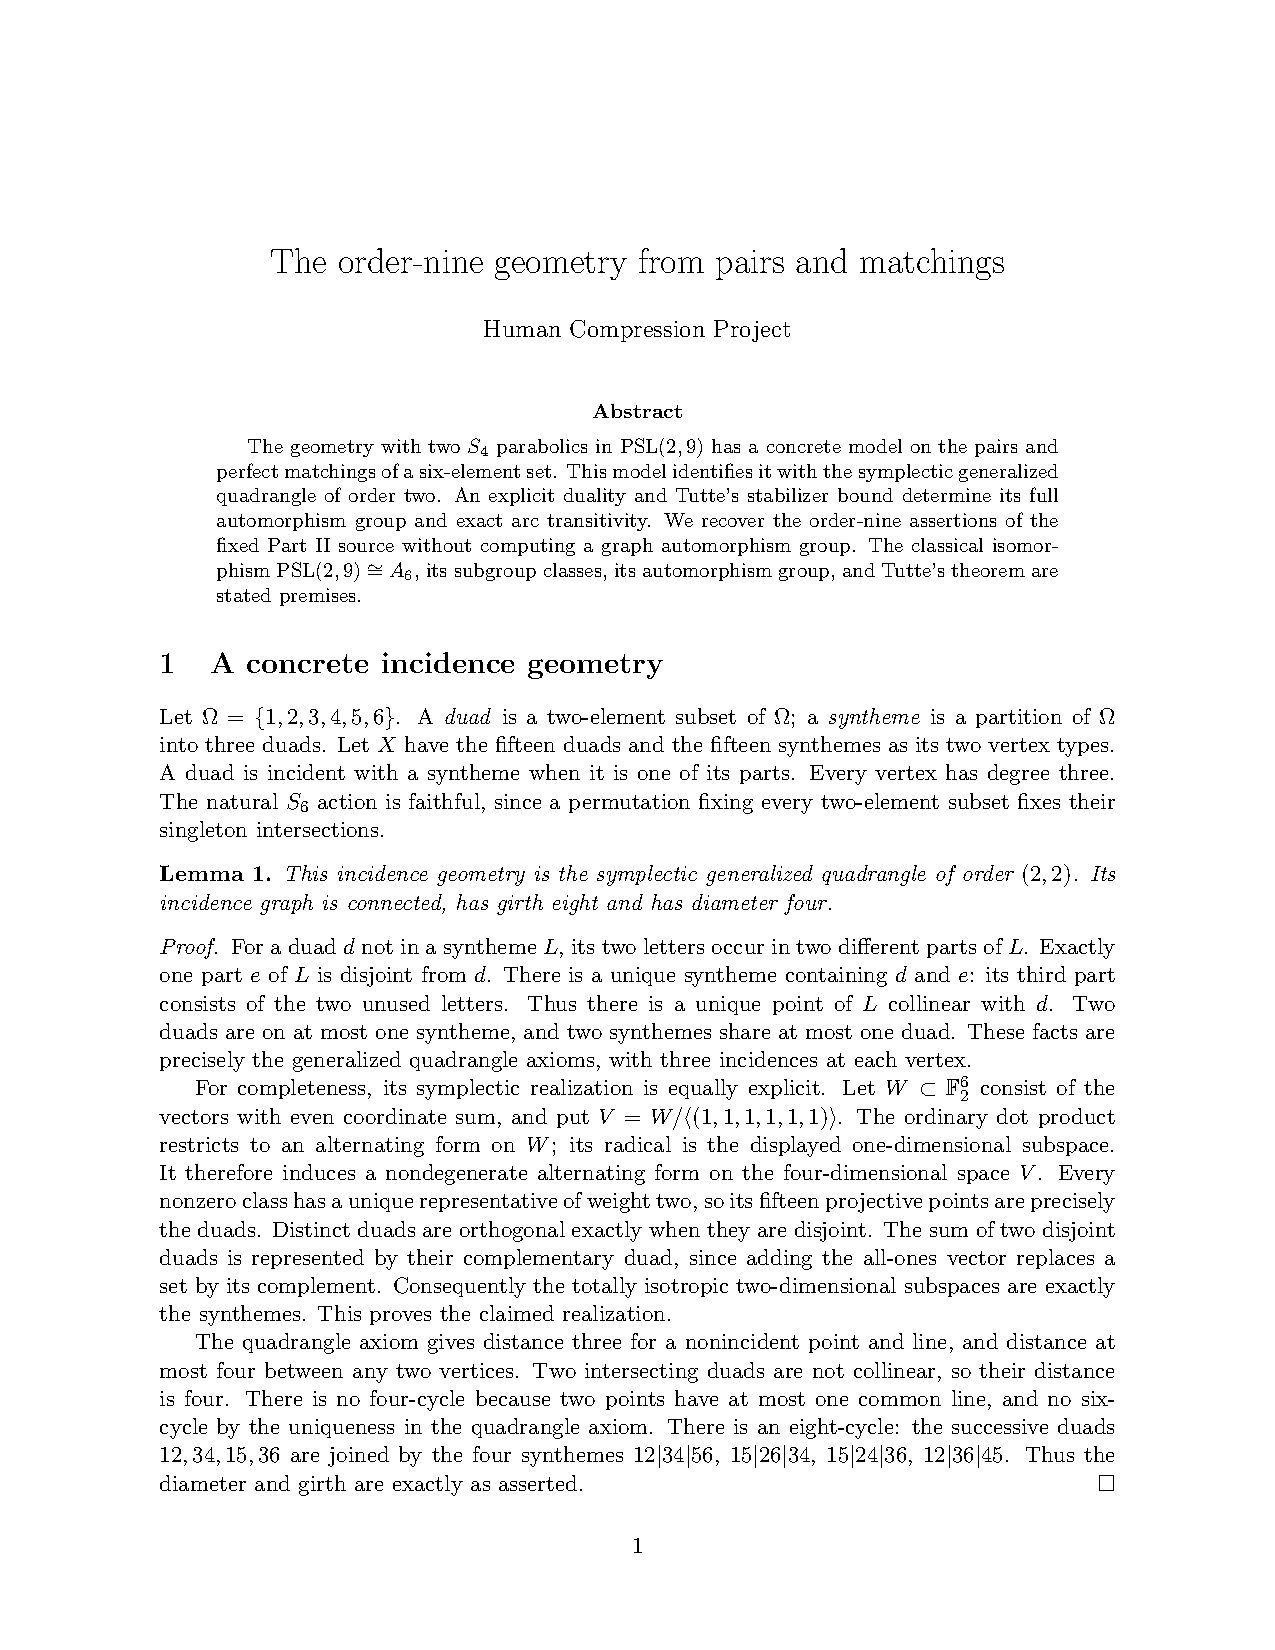
\includepdf[pages=-]{proofs/q9.pdf}
\end{document}
